\section{Réciproque du théorème de Thalès}
    \subsection{Énoncé}
        \begin{theoreme}[\admis]
            Si dans un triangle $ABC$ :
            \begin{itemize}
                \item $M$ est un point du côté $[AB]$ distinct de $A$ et $B$.
                \item $N$ est un point du côté $[AC]$ distinct de $A$ et $C$.
                \item $\dfrac{AM}{AB} = \dfrac{AN}{AC}$.       
            \end{itemize}
            \medskip
            alors les droites $(BC)$ et $(MN)$ sont parallèles.
        \end{theoreme}

    \subsection{Exemple de rédaction}

        \begin{methode*1}[Justifier que deux droites sont parallèles]
            \begin{multicols}2
                \begin{itemize}
                    \item Identifier les deux triangles.                                    
                    \item Calculer les rapports de longueurs non portées par les droites candidates.
                    \item Invoquer la réciproque du théorème de Thalès.
                \end{itemize}
            \end{multicols}

            \exercice

            \begin{minipage}{8cm}
                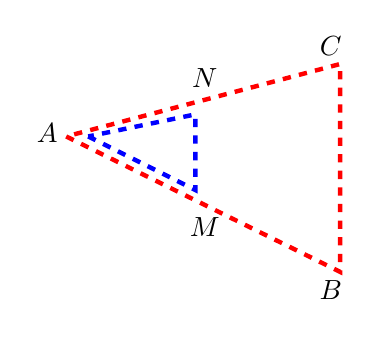
\begin{tikzpicture}[scale = 0.4]
                    \begin{scope}[rotate=90]
                    % \draw[help lines, color=black!30, dashed] (0,0) grid (12,18);        
                    \coordinate[label={[xshift=-4mm, yshift=-2mm]$A$}] (A) at (7,13);                    
                    \coordinate[label={[xshift=0mm, yshift=1mm]$C$}] (C) at (9,5);
                    \coordinate[label={[xshift=0mm, yshift=-6mm]$B$}] (B) at (3,5);
                    \coordinate[label={[xshift=0mm, yshift=-6mm]$M$}] (M) at (5,9);
                    \coordinate[label={[xshift=0mm, yshift=1mm]$N$}] (N) at (8,9);
                    \coordinate (A1) at (7,12.7);
                    \coordinate (A2) at (7,13.4);
                    \coordinate (B1) at (2.7,4.7);
                    \coordinate (C1) at (9.3,4.7);
                    \coordinate (M1) at (5.3,9.3);
                    \coordinate (N1) at (7.7,9.3);
                    \tkzDrawSegment[ultra thick](A,B);
                    \tkzDrawSegment[ultra thick](A,C);
                    \tkzDrawSegment[ultra thick](M,N);
                    \tkzDrawSegment[ultra thick](B,C);                    
                    \draw[dashed, color=blue, ultra thick] (A1)--(M1)--(N1)--(A1);
                    \draw[dashed, color=red, ultra thick] (A2)--(B1)--(C1)--(A2);
                    \end{scope}
                \end{tikzpicture}
            \end{minipage}
            \begin{minipage}{8cm}
                \begin{itemize}
                    \item Les droites $(d)$ et $(d')$ se coupent en $A$.
                    \item $AB=\Lg{9}$ ; $AM=\Lg{5.4}$.
                    \item $AC=\Lg{12.5}$ ; $AN=\Lg{7.5}$.
                \end{itemize}

                % \vspace*{1cm}
                Démontrer que les droites $(MN)$ et $(BC)$ sont parallèles.
            \end{minipage}
            
            \correction
            Dans la configuration ci-dessus : 
            \begin{itemize}               
                \item les deux triangles sont \textcolor{blue}{$AMN$} et \textcolor{red}{$ABC$}.
                \item $M \in [AB]$ et $N \in [AC]$.
                \medskip
                \item D'une part $\dfrac{\textcolor{blue}{AM}}{\textcolor{red}{AB}} = \dfrac{\textcolor{blue}{5,4}}{\textcolor{red}{9}}=0,6$
                \hfill
                D'autre part $\dfrac{\textcolor{blue}{AN}}{\textcolor{red}{AC}} = \dfrac{\textcolor{blue}{7,5}}{\textcolor{red}{12,5}}=0,6$
            \end{itemize}
            On constate que $\dfrac{AM}{AB} = \dfrac{AN}{AC}$, d'après la réciproque du théorème de Thalès, on peut conclure que \psshadowbox{les droites $(MN)$ et $(BC)$ ne sont pas parallèles}.
        \end{methode*1}
